\documentclass{article}
\usepackage{
	amsmath,			% Math Environments
	amssymb,			% Extended Symbols
	enumerate,		    % Enumerate Environments
	graphicx,			% Include Images
        minted,
        caption,
        subcaption,
        booktabs,
        microtype,
}
\usepackage[norsk]{babel}
\usepackage[T1]{fontenc}
\usepackage{hyperref}
\hypersetup{breaklinks=true,colorlinks=true,linkcolor=blue,citecolor=blue,filecolor=magenta,urlcolor=blue}
% \bibliographystyle{apalike}
\bibliographystyle{IEEEtran}

\renewcommand{\thesection}{Oppgave \arabic{section}}
\renewcommand{\thesubsection}{\arabic{section}\alph{subsection})}
\renewcommand{\thesubsubsection}{Besvarelse}

\setminted{
tabsize=4,
fontsize=\footnotesize,
%style=tango,
%style=autumn,
%style=lovelace,
% style=numpy,
% style=abap,
%bgcolor=gray,  %background color
%fontsize= ,
linenos,        %line number
breaklines      % allow word wrap for code
}

\title{MAT1020 - Oblig 1\\Matematikk og bærekraftig forvaltning}
\author{August Femtehjell}
\date{March 2024}

\begin{document}

\maketitle

\noindent
All koden for denne obligen er tilgjengelig på \url{https://github.com/augustfe/MAT1020}, skrevet i \verb|Python|.

\section{}
I denne oppgaven skal du gjøre en statistisk analyse av kapasitetsfaktordataene.

\subsection{}
Plot alle dataseriene (gjerne som illustrative utsnitt av tidsseriene), og se om det er forskjeller mellom årstidene. Hva kan du si om solkraft nord og sør i Europa og vindkraft på de forskjellige stedene i Norge?

\subsubsection{}
Etter som solkapasitetene er gitt ved maskimalverdier klokken 12, er vi nødt til å gjøre justeringer for å få representative daglige verdier.
Hvis vi antar at gjennomsnitts solkapasiteten er gitt ved halvparten av maks, og at det er 12 timer med sol hver dag, ganger vi de gitte solkapasitetene med $\frac{1}{4}$ for å justere.
Det kan diskuteres hvorvidt dette er en representativ måte å bearbeide dataen, spesielt med tanke på at antall soltimer i løpet av et døgn varierer med tiden av året, og lokasjon.
Oslo ligger for eksempel på rundt 1700 timer med sol hvert år, mens Athen ligger på omtrent 2800 \cite{soltimer}.

For å få et inntrykk av hva slags data vi jobber med, plotter jeg tidsseriene uten videre justeringer i \autoref{fig:rene_tidserier}, ved hjelp av \verb|Pandas| sitt \verb|DataFrame|.
Som en kan se, er dette ikke særlig illustrativt, på grunn av de store daglige svingningene, annet enn at solkapasitet angivelig varierer med årstid.

\begin{figure}[ht]
\centering
\begin{subfigure}{.5\textwidth}
    \centering
    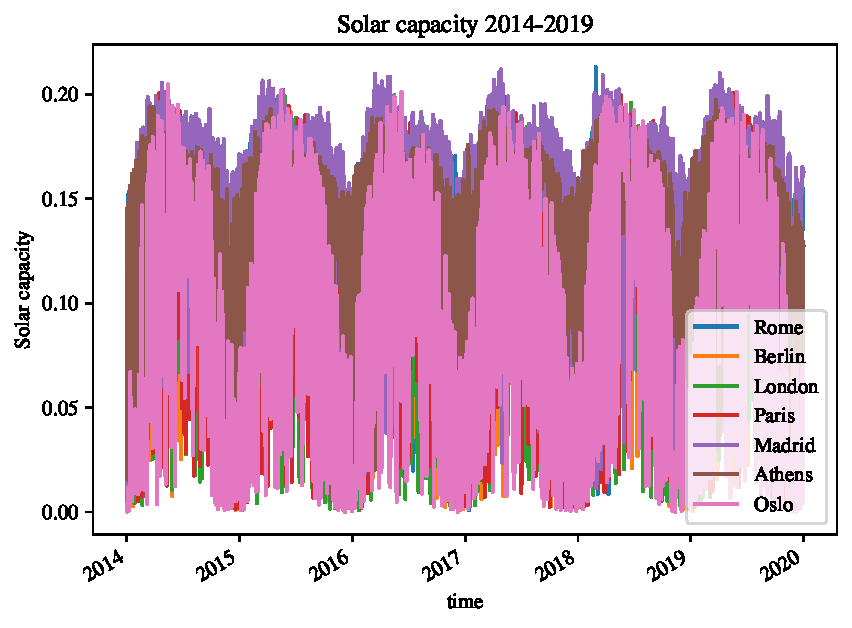
\includegraphics[width=\linewidth]{figures/Solar/Solar capacity 2014-2019.pdf}
    \caption{Solkapasitet}
    \label{fig:ren_sol}
\end{subfigure}%
\begin{subfigure}{.5\textwidth}
    \centering
    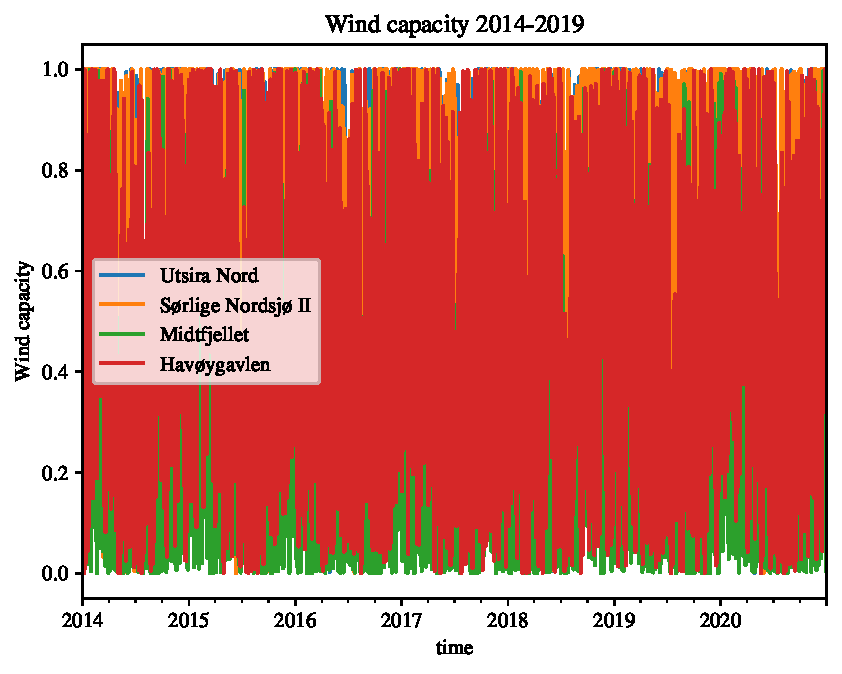
\includegraphics[width=\linewidth]{figures/Wind/Wind capacity 2014-2019.pdf}
    \caption{Vindkapasitet}
    \label{fig:ren_vind}
\end{subfigure}
\caption{Tidsserier for sol- og vindkapasitet.}
\label{fig:rene_tidserier}
\end{figure}

For å få et bedre bilde, velger jeg derfor å benytte meg av et løpende gjennomsnitt på 30 dager, ved \verb|DataFrame.rolling(30).mean|, for å luke ut de mindre daglige svingingene.
I tillegg, så velger jeg å fokusere på et enkelt år, hvor 2017 er valgt arbitrært.
I \autoref{fig:rolling_2017_sol} kan vi nå tydeligere se at solkapasitetene varierer sterkt fra by til by, med høyere kapasitet i sør og lavere i nord.
Med vindkapasitetene i \autoref{fig:rolling_2017_vind}, skiller Midtfjellet seg sterkt ut fra de andre lokasjonene.

\begin{figure}[ht]
\centering
\begin{subfigure}{.5\textwidth}
    \centering
    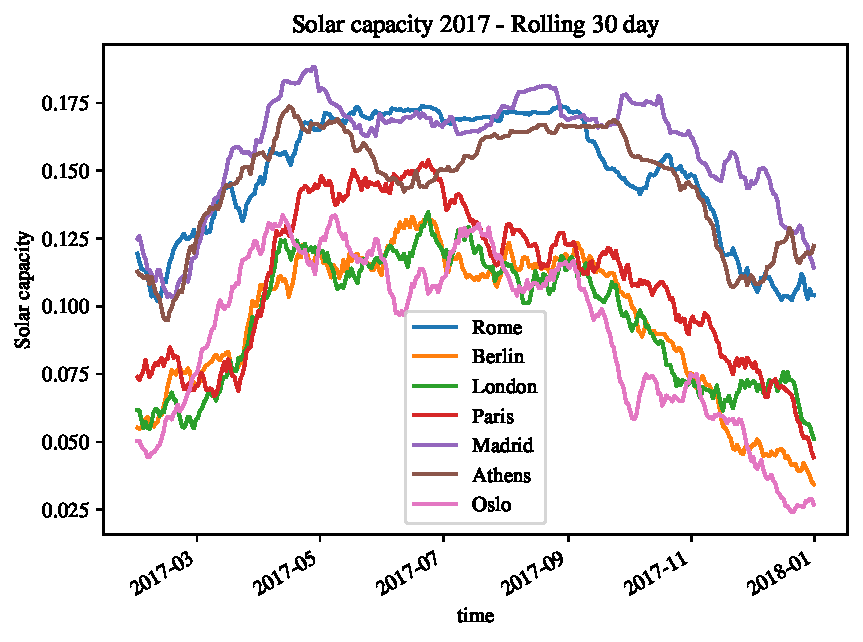
\includegraphics[width=\linewidth]{figures/Solar/Solar capacity 2017 - Rolling 30 day.pdf}
    \caption{Solkapasitet}
    \label{fig:rolling_2017_sol}
\end{subfigure}%
\begin{subfigure}{.5\textwidth}
    \centering
    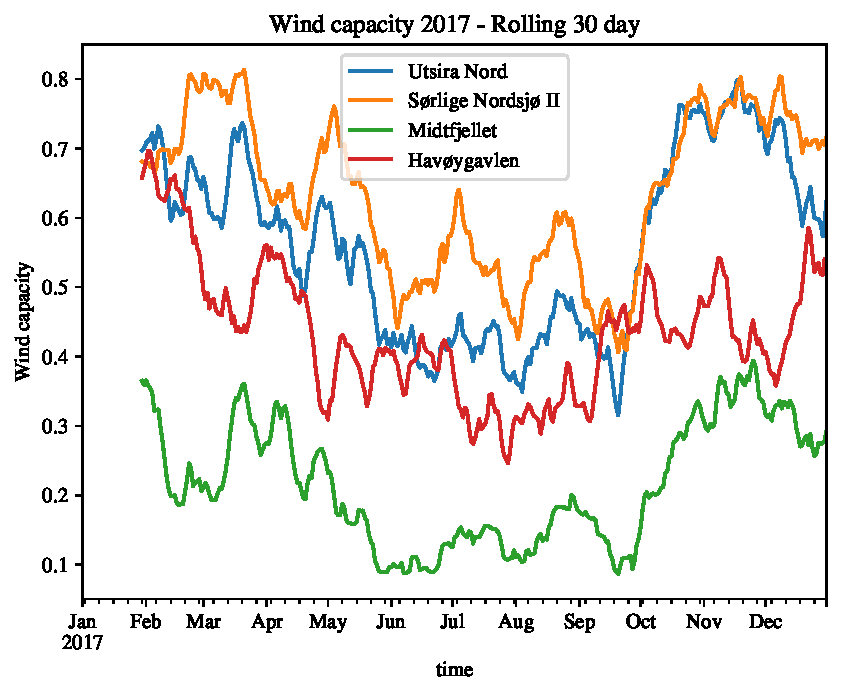
\includegraphics[width=\linewidth]{figures/Wind/Wind capacity 2017 - Rolling 30 day.pdf}
    \caption{Vindkapasitet}
    \label{fig:rolling_2017_vind}
\end{subfigure}
\caption{Løpende gjennomsnitt over 30 dager, for sol- og vindkapasitet i 2017.}
\label{fig:rolling_2017}
\end{figure}

\newpage
\subsection{}
Finn gjennomsnittlig kapasitetsfaktor for hver sol- og vind-dataserie. Husk å omforme sol-dataene til representative daglige verdier.

\subsubsection{}
De gjennomsnittlige kapasitetsfaktorene er oppgitt i \autoref{tab:gjennomsnitt_tabell}, merk at soldataen allerede er justert til mer representative daglige verdier.
Koden for utregning finnes i \autoref{sec:oppg1}.

\begin{table}[h]
\centering
\subfloat[Solkraft]{
    \begin{tabular}{l|r}
    \toprule
    \midrule
    Roma     & 0.138063 \\
    Berlin   & 0.098143 \\
    London   & 0.096166 \\
    Paris    & 0.107171 \\
    Madrid   & 0.149532 \\
    Athen   & 0.139312 \\
    Oslo     & 0.087412 \\
    \bottomrule
    \end{tabular}
}
\qquad
\subfloat[Vindkraft]{
    \begin{tabular}{l|r}
    \toprule
    \midrule
    Utsira Nord          & 0.571073 \\
    Sørlige Nordsjø II   & 0.640919 \\
    Midtfjellet          & 0.243222 \\
    Havøygavlen          & 0.469817 \\
    \bottomrule
    \end{tabular}
    }
\caption{Gjennomsnittlige kapasitetsfaktorer per lokasjon og teknologi.}
\label{tab:gjennomsnitt_tabell}
\end{table}

Her blir forskjellene mellom regionene mer markante, blant annet ved at madrid i sør har en $1.71$ ganger høyere gjennomsnittlig kapasitetsfaktor enn Oslo i Nord, og at off-shore installasjonen Sørlige Nordsjø II har en $2.64$ ganger høyere kapasitetsfaktor enn Midtfjellet.

\subsection{}
Finn varians og standardavvik for kapasitetsfaktorene i hver lokasjon og hver teknologi (det vil si, sol og vind)

\subsubsection{}
Standardavvikene er oppgitt i \autoref{tab:std_tabell}.
Standardavviket i Oslo er betydelig høyere enn for eksempel Athen, som gir mening ettersom det er betydelig mindre sol i Oslo om vinteren enn det er i Athen.
Solkraft har dog betydelig lavere standardavvik enn vindkraft. Utregningen er beskrevet i \autoref{sec:oppg1}, med variansen oppgitt langs diagonalen i \autoref{fig:covariance}.

\begin{table}[h]
\centering
\subfloat[Solkraft]{
\begin{tabular}{l|r}
    \toprule
    \midrule
    Roma & 0.043663 \\
    Berlin & 0.054475 \\
    London & 0.053795 \\
    Paris & 0.057088 \\
    Madrid & 0.046485 \\
    Athen & 0.039253 \\
    Oslo & 0.061271 \\
    \bottomrule
\end{tabular}
}
\qquad
\subfloat[Vindkraft]{
\begin{tabular}{l|r}
    \toprule
    \midrule
    Utsira Nord & 0.330635 \\
    Sørlige Nordsjø II & 0.315474 \\
    Midtfjellet & 0.266767 \\
    Havøygavlen & 0.315342 \\
    \bottomrule
\end{tabular}
}
\caption{Standardavvik for kapasitetsfaktorer per lokasjon og teknologi.}
\label{tab:std_tabell}
\end{table}

\begin{figure}[h]
\centering
\begin{subfigure}{.5\textwidth}
    \centering
    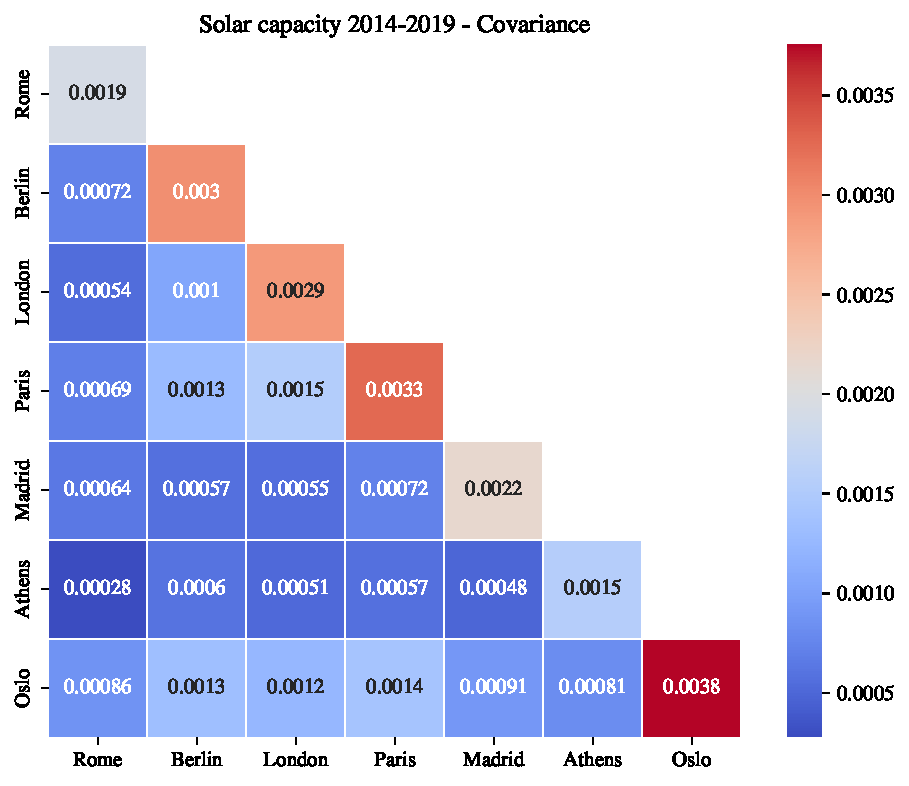
\includegraphics[width=\linewidth]{figures/Solar/Solar capacity 2014-2019 - Covariance.pdf}
    \caption{Solkapasitet}
    \label{fig:cov_sol}
\end{subfigure}%
\begin{subfigure}{.5\textwidth}
    \centering
    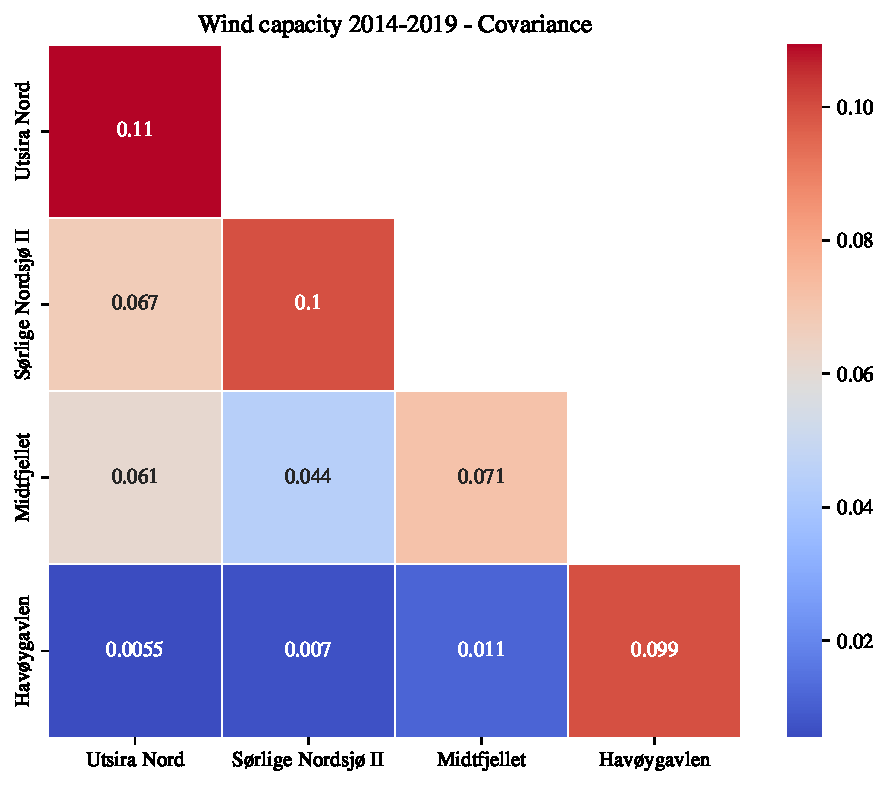
\includegraphics[width=\linewidth]{figures/Wind/Wind capacity 2014-2019 - Covariance.pdf}
    \caption{Vindkapasitet}
    \label{fig:cov_vind}
\end{subfigure}
\caption{Kovarians mellom lokasjoner, for hver teknologi.}
\label{fig:covariance}
\end{figure}


\newpage
\subsection{}
Finn kovariansen til kapasitetsfaktorene mellom lokasjoner for vind. Hva blir korrelasjonene?

\subsubsection{}
I \autoref{fig:cov_vind} kan vi lese at det er absolutt minst korrelasjon mellom Havøygavlen og de andre.
Dette gir mening, ettersom Havøygavlen ligger i Finnmark, mens eksempelvis Midtfjellet ligger på vestlandet. Det er dog høy korrelasjon mellom Utsira Nord og Midtfjellet.
Korrelasjonene er oppgitt i \autoref{fig:corr_vind}, utregnet i \autoref{sec:oppg1}.

\begin{figure}[h]
\centering
\begin{subfigure}{.5\textwidth}
    \centering
    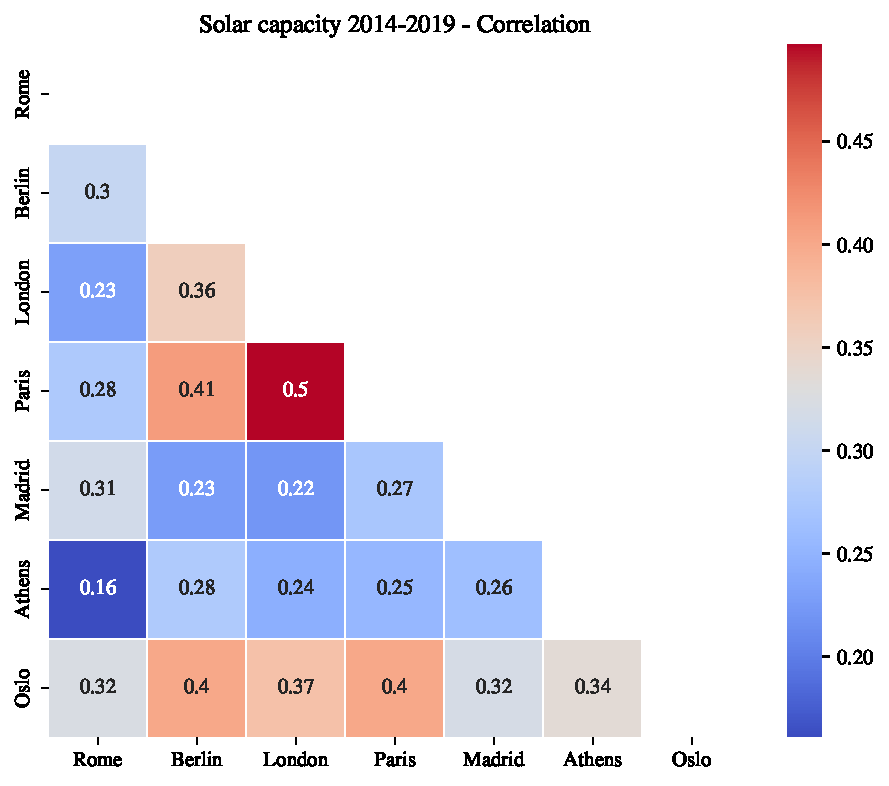
\includegraphics[width=\linewidth]{figures/Solar/Solar capacity 2014-2019 - Correlation.pdf}
    \caption{Solkapasitet}
    \label{fig:corr_sol}
\end{subfigure}%
\begin{subfigure}{.5\textwidth}
    \centering
    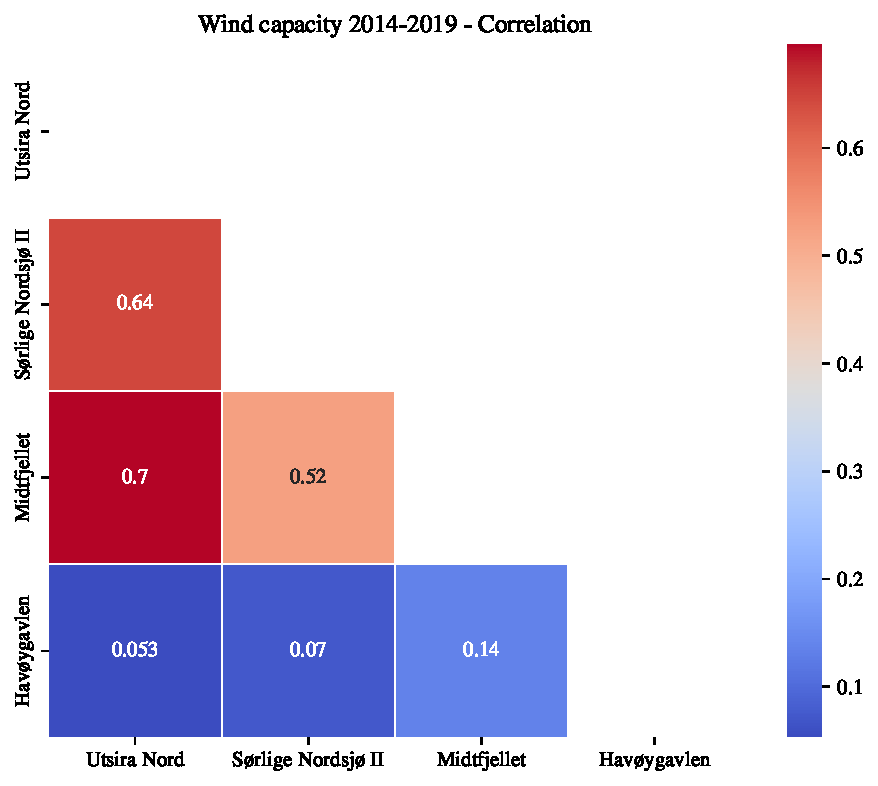
\includegraphics[width=\linewidth]{figures/Wind/Wind capacity 2014-2019 - Correlation.pdf}
    \caption{Vindkapasitet}
    \label{fig:corr_vind}
\end{subfigure}
\caption{Korrelasjoner mellom lokasjoner, for hver teknologi.}
\label{fig:correlation}
\end{figure}

\subsection{}
Finn kovariansen til kapasitetsfaktorene mellom lokasjoner for sol. Hva blir korrelasjonene?

\subsubsection{}
I \autoref{fig:cov_sol} kan vi lese av kovariansen til solkapasitetene mellom byene i Europa.
Det er betraktelig lavere kovarians i denne settingen, dog høyere mellom byer som Paris og London.
Dette gir mening ettersom det er omtrentlige 344km mellom de, mot 2600km mellom Oslo og Athen.
Korrelasjonene er oppgitt i \autoref{fig:corr_sol}.

\subsection{}
Finn varians-kovariansmatrisen for kapasitetsfaktorene til sol og for kapasitetsfaktorene til vind.

\subsubsection{}
For ordens skyld er varians-kovariansmatrisen for sol oppgitt i \autoref{tab:var_cov_sol} og vind i \autoref{tab:var_cov_vind}. Merk at dette ble svært lite lesbart, og inneholder den samme informasjonen som \autoref{fig:covariance}. Verdiene er utregnet ved hjelp av koden i \autoref{sec:oppg1}.

\begin{table}[h]
\centering
$$
\begin{bmatrix}
0.001906 & 0.000715 & 0.000539 & 0.000689 & 0.000637 & 0.000276 & 0.000863 \\
0.000715 & 0.002968 & 0.001045 & 0.001277 & 0.000571 & 0.000595 & 0.001335 \\
0.000539 & 0.001045 & 0.002894 & 0.001526 & 0.000551 & 0.000515 & 0.001232 \\
0.000689 & 0.001277 & 0.001526 & 0.003259 & 0.000720 & 0.000568 & 0.001400 \\
0.000637 & 0.000571 & 0.000551 & 0.000720 & 0.002161 & 0.000479 & 0.000908 \\
0.000276 & 0.000595 & 0.000515 & 0.000568 & 0.000479 & 0.001541 & 0.000807 \\
0.000863 & 0.001335 & 0.001232 & 0.001400 & 0.000908 & 0.000807 & 0.003754 \\
\end{bmatrix}
$$
\caption{Varians-kovariansmatrisen for kapasitetsfaktorene til sol, i samme rekkefølge som \autoref{tab:gjennomsnitt_tabell}.}
\label{tab:var_cov_sol}
\end{table}

\begin{table}[h]
\centering
$$
\begin{bmatrix}
0.109319 & 0.067227 & 0.061392 & 0.005485 \\
0.067227 & 0.099524 & 0.044098 & 0.006990 \\
0.061392 & 0.044098 & 0.071165 & 0.011390 \\
0.005485 & 0.006990 & 0.011390 & 0.099441 \\
\end{bmatrix}
$$
\caption{Varians-kovariansmatrisen for kapasitetsfaktorene til vind, i samme rekkefølge som \autoref{tab:gjennomsnitt_tabell}.}
\label{tab:var_cov_vind}
\end{table}

\newpage
\section{}
Du skal i denne oppgaven finne den beste mulige installeringen av solcelleparker og vindparker som gir minst mulig variasjon rundt etterspørselen etter strøm.
Du skal analysere vindparker og solcelleparker hver for seg, og anta at lokasjonene du kan bygge fornybar kraft er gitt som i dataene i oppgave 1.
Vi tenker oss at etterspørselen etter kraft er konstant, slik at variansen $\hat{\sigma}_E^2 = 0$.
Når du skal analysere solkraft i Europa, skal du anta at etterspørselen er $\hat{\mu}_E = 100$GWh i en time, mens vindkraft i Norge er på $1$GWh.
Disse to tallene er etterspørselen i en \textit{typisk} time på en dag, og du kan basere deg på gjennomsnittlig kapasitetsfaktor for den aktuelle dagen nå du skal beregne produksjonen i en \textit{typisk} time på en dag.
Du skal altså minimere produksjonens variasjon i en \textit{typisk} time rundt den etterspørselen som er oppgitt.

\subsection{}
Finn optimal installering av solkraft i Europa og vindkraft i Norge.
Finner du noen lokasjoner det installeringen blir negativ?
Hvis så er tilfelle, luk ut disse, og gjør analysen på nytt.
Eventuelt, bruk optimeringsverktøy der du kan legge inn krav om positive verdier av $\mathbf{w}$.

\subsubsection{}
Vi finner den optimale installeringen ved å løse optimeringsproblemet
\begin{equation}
\begin{array}{clcc}
    \min\limits_{\mathbf{W} \in \mathbb{R}^d} & \mathbf{w}^T C \mathbf{w} + \left( \mathbf{w}^T \hat{\mathbf{r}} - \hat{\mu}_E \right)^2 + \hat{\sigma}_E^2, \\
    \text{gitt at} & \mathbf{w} \geq 0.
\end{array}
\end{equation}
$\hat{\mu}_E$ tilsvarer den ønskede kapasiteten, altså $100$GWh for solkraft og $1$GWh for vindkraft, gitt de gjennomsnittlige kapasitetsfaktorene $\hat{\mathbf{r}}$.
$\mathbf{w}$ blir da nødvendig installert kapasitet for hver av de $d$ stasjonene.
$C$ er varians-kovariansmatrisen for de forskjellige lokasjonene, og $\hat{\sigma}_E^2$ er variansen til etterspørselen, som vi antar at er null.

Jeg løser dette ved å bruke \verb|scipy.optimize.minimize| i \verb|Python|, for å påse at $\mathbf{w} \geq 0$, beskrevet i \autoref{sec:oppg2}.
De optimale verdiene for solkraft er oppgitt i GW i \autoref{tab:kapasitet_sol}, mens verdiene for vindkraft er oppgitt i MW i \autoref{tab:kapasitet_vind_MW}. For ordens skyld er de og oppgitt i GW i \autoref{tab:kapasitet_vind_GW}.

\begin{table}[h]
\centering
\subfloat[Solkraft i GW]{
\begin{tabular}{l|r}
\toprule
\midrule
Roma & 206.45 \\
Berlin & 0.00 \\
London & 20.19 \\
Paris & 0.22 \\
Madrid & 164.99 \\
Athen & 291.34 \\
Oslo & 0.00 \\
\midrule
Total & 683.19 \\
\bottomrule
\end{tabular}
\label{tab:kapasitet_sol}
}
\\
\subfloat[Vindkraft i MW]{
\begin{tabular}{l|r}
\toprule
\midrule
Utsira Nord & 291.66 \\
Sørlige Nordsjø II & 651.48 \\
Midtfjellet & 0.00 \\
Havøygavlen & 591.07 \\
\midrule
Total & 1534.20 \\
\bottomrule
\end{tabular}
\label{tab:kapasitet_vind_MW}
}
\qquad
\subfloat[Vindkraft i GW]{
\begin{tabular}{l|r}
\toprule
\midrule
Utsira Nord & 0.29 \\
Sørlige Nordsjø II & 0.65 \\
Midtfjellet & 0.00 \\
Havøygavlen & 0.59 \\
\midrule
Total & 1.53 \\
\bottomrule
\end{tabular}
\label{tab:kapasitet_vind_GW}
}
\caption{Optimal installering per teknologi.}
\label{tab:kapasitet}
\end{table}

\newpage
\subsection{}
Hva blir den minste produksjonsvariasjonen rundt etterspørselen du kan oppnå?

\subsubsection{}
Den minste oppnåelige produksjonsvariansen ble
\begin{equation}
    L(\bar{\mathbf{w}}_{\text{sol}}) = 427.38 \qquad \text{og} \qquad L(\bar{\mathbf{w}}_{\text{vind}}) = 0.14,
\end{equation}
ved hjelp av \verb|quadprog| fra \autoref{sec:oppg2}.

\subsection{}
Finn beste installering i enkelt-lokasjoner som minimerer variasjonen rundt etterspørselen.
Hva blir produksjonvariasjonen rundt etterspørselen, og hvor mye kan du redusere denne (i prosent) med å installere i flere lokasjoner?

\subsubsection{}
De laveste produksjonsvariansene vi kan oppnå med én lokasjon er $735.50$ for solkraft i Athen og $0.20$ for vind fra Sørlige Nordsjø II.
Tabellen med resultatene for de andre lokasjonene er oppgitt i \autoref{tab:prod_var_sol}.
Vi får dermed en reduksjon på henholdsvis $41.89\%$ og $29.14\%$ ved å installere ved flere lokasjoner.
Disse verdiene ble utregnet ved hjelp av \verb|single_installement| fra \autoref{sec:oppg2}.

\begin{table}[h]
\centering
\subfloat[Solkapasitet]{
\begin{tabular}{l|r|r}
    \toprule
     & Produksjons- & Nødvendig \\
     & varians & kapasitet \\
    \midrule
    Roma & 909.23 & 658.45 \\
    Berlin & 2355.29 & 778.94 \\
    London & 2383.43 & 792.02 \\
    Paris & 2210.35 & 726.85 \\
    Madrid & 881.24 & 609.82 \\
    Athen & 735.50 & 665.02 \\
    Oslo & 3294.55 & 767.10 \\
    \bottomrule
\end{tabular}
}
\quad
\subfloat[Vindkapasitet]{
\begin{tabular}{l|r|r}
\toprule
& Produksjons- & Nødvendig \\
     & varians & kapasitet \\
\midrule
Utsira Nord & 0.25 & 1.31 \\
Sørlige Nordsjø II & 0.20 & 1.26 \\
Midtfjellet & 0.55 & 1.87 \\
Havøygavlen & 0.31 & 1.47 \\
\bottomrule
\end{tabular}
}
\caption{Produksjonsvarians og nødvendigkapasitet ved enkelt-lokasjoner per teknologi.}
\label{tab:prod_var_sol}
\end{table}

\subsection{}
Regn ut forventet produksjon for de ulike installeringsbeslutningene du har gjort i a) og c).
Kommenter svarene dine.

\subsubsection{}
Vi finner forventet produksjon ved å multiplisere optimal bygd kapasitet vi fant, med forventet sol- og vindkapasitet, oppgitt i \autoref{tab:expected}.
Utregningen ble gjort via \verb|expected_production| fra \autoref{sec:oppg2}.
I alle scenarier er forventet produksjon under den forventede etterspørsellen.
Dette kommer av at vi ikke kun vil minimere tilfeller hvor vi produserer for lite strøm, men også når vi produserer for mye.

\begin{table}[h]
\centering
\subfloat[Solkraft]{
\begin{tabular}{l|r}
    \toprule
     & Forventet \\
     & produksjon \\
    \midrule
    Roma & 90.91 \\
    Berlin & 76.45 \\
    London & 76.17 \\
    Paris & 77.90 \\
    Madrid & 91.19 \\
    Athen & 92.64 \\
    Oslo & 67.05 \\
    \bottomrule
    Optimal & 95.73 \\
    \bottomrule
\end{tabular}
}
\qquad
\subfloat[Vindkraft]{
\begin{tabular}{l|r}
    \toprule
     & Forventet \\
     & produksjon \\
    \midrule
    Utsira Nord & 0.75 \\
    Sørlige Nordsjø II & 0.80 \\
    Midtfjellet & 0.45 \\
    Havøygavlen & 0.69 \\
    \bottomrule
    Optimal & 0.86 \\
    \bottomrule
\end{tabular}
}
\caption{Forventet produksjon for de ulike installeringsbeslutningene, per teknologi.}
\label{tab:expected}
\end{table}

Vi hadde kun fått en reduksjon i produksjon på henholdsvis $3.2\%$ og $7.0\%$ ved å plassere all produksjonen i de mest optimale enkelt installasjonene, men som diskutert tidligere er endringene i produksjonsvarians mye større.

Vi kommer altså absolutt tettest på den forventede etterspørselen med minst produksjonsvarians ved å benytte oss av flere lokasjoner.

\newpage
\subsection{}
Hvis du skulle ha utført utbyggingen av sol og vindkraft i praksis, hva måtte du ha tatt hensyn til av sosiale, politiske, økonomiske og tekniske forhold?

\subsubsection{}
Det mest åpenbare i forhold til hva en måtte tatt hensyn til i forhold til utbygging av vindkraft i Norge, er kanskje hva de ulike partiene mener om det.
Med utgangspunkt i partiprogrammene for 2021, så er de fleste partiene generelt sett negative til vindkraft på land \cite{nrk_vindkraft}.
De største partiene, Høyre og Arbeiderpartiet, er dog angivelig mer positive til vindkraft.
Angivelig så satser Høyre på \textit{``lønnsomme, fornybare prosjekter''} \cite{nrk_vindkraft}, men utbroderer ikke i stor grad om hvordan vindkraft på land skal håndteres, annet enn at kommunene skal kunne bestemme selv \cite{høyre_vindkraft}.
Arbeiderpartiet på sin side setter et fokus på at \textit{``Vi trenger mer kraft''} \cite{ap_vindkraft}, og at dette skal oppnås ved blant annet \textit{``et strengere regime for utbygging av vindkraft på land''} \cite{nrk_vindkraft}.

De andre partiene siterer i varierende grad bekymringer rundt naturvern og kommuners selvbestemmelse for hvorfor de er negative til vindkraft på land.
Med havvind er det derimot større entusiasme, med unntak av Rødt som fremdeles siterer naturvern som grunn til å være i mot \cite{nrk_vindkraft}.

Stortinget vedtok 21.03.2024 at Regjeringen skal sette et mål om 8TWh med ny solkraft innen 2030, innen revidert statsbudsjett for 2024, etter forslag fra SVs Lars Haltbrekken og Kari Elisabeth Kaski \cite{representant_sol}.
Dette målet skal blant annet oppnås gjennom særskilte skatteregler for salg av overskuddsstrøm, slik at produksjon under boligens årsforbruk ikke skattelegges.

Installasjon av vindkraft innebærer store miljømessige inngrep, enten det installeres til havs eller på land.
En av hovedgrunnene til at vi i det hele tatt er interesserte i bygge ut mer fornybar energi, er for å redusere klimagassutslipp.
Det er ingen selvfølge at et regnestykke om å bygge et vindkraftanlegg vil slå ut positivt.
NRK avdekket blant annet at myr som karbonlager ikke hadde blitt medberegnet i konsekvensutredningene til 88 vindkraftverk \cite{myr_vindkraft}.
En annen bekymring som ofte nevnes i forbindelse med vindkraft, er effekten det kan ha på fugleliv.
Dette kan mitigeres ved å, blant annet, benytte seg av ny teknologi for å detektere kollisjoner \cite{spoor}, eller ved å ta hensyn til fuglers migrasjonsmønster i utbyggingen av nye anlegg \cite{NINA_migration}.

I tillegg er vindkraftinstallasjoner sjeldent fine å se på, som ofte fører til stor motstand blant innbyggerne rundt anleggene.
Dette har som konsekvens at selv om de fleste er enige i at vi må bygge mer fornybart, så har det en tendens til å \textit{bare ikke passe akkurat her}.
En måte å motivere kommuner til å bygge fornybart, er derfor ved å tilby økonomiske insentiver, ofte i form av billigere strøm.

Av tekniske forhold er det naturlig å ta hensyn til blant annet kapasitetsfaktorer, i samme art av hva som er blitt gjort tidligere i denne oppgaven, for å få effektiv utnyttelse av de anleggene som bygges.
Et annet viktig aspekt, er at kraften som produseres er nødt til å bli fraktet til der den skal utnyttes.
Det er derfor lite hensiktsmessig å bygge et ekstremt effektivt anlegg, med mindre det er noen i nærheten som kan ta nytte av den, eller det finnes infrastruktur for å frakte energien.
For at tungtransport skal kunne elektrifiseres, er vi avhengige av et effektivt ladenettverk langs hele Norge.
Statens vegvesen har derfor utredet muligheten for å bygge solkraft langs veiene \cite{vegvesen}.
Dette er gunstig av flere grunner, som at vegvesenet ofte er grunneiere langs veiene og områdene rundt, som kan lette på byråkratiet som ofte preger utbygging, i tillegg til at den nødvendige infrastrukturen sjeldent er langt unna.
Tunneller har blant annet et ekstremt effektbehov ved brann, og har derfor god nettilknytning \cite{edvard}.



\bibliography{references}
\appendix
\section{Kode til Oppgave 1}\label{sec:oppg1}
\begin{minted}{numpy}
# Omform til representative verdier
solar_df: DataFrame = raw_solar / 4

# Gjennomsnitt
mean_solar = solar_df.mean()
mean_wind = wind_df.mean()

# Standardavvik
std_solar = solar_df.std()
std_wind = wind_df.std()

# Varians
var_solar = solar_df.var()
var_wind = wind_df.var()

# Kovarians
var_solar = solar_df.cov()
var_wind = wind_df.cov()

# Korrelasjon
corr_solar = solar_df.corr()
corr_wind = wind_df.corr()
\end{minted}

\section{Kode til Oppgave 2}\label{sec:oppg2}

\begin{minted}{numpy}
def objective_func(
    w: np.ndarray, C: np.ndarray, E_demand: float, r: np.ndarray
) -> float:
    """Quadprog function to minimize. This function is the objective function for the quadratic programming problem.

    Args:
        w (np.ndarray): Weights of the installed capacity
        C (np.ndarray): Covariance matrix of the locations
        E_demand (float): Expected demand
        r (np.ndarray): Expected capacity factors of the locations

    Returns:
        float: The value of the objective function
    """
    return w.T @ C @ w + (w @ r - E_demand) ** 2


def quadprog(X: DataFrame, E_demand: float) -> tuple[np.ndarray, float]:
    """Find the optimal weights for the installed capacity using quadratic programming.

    Args:
        X (DataFrame): DataFrame of the capacity factors of the locations
        E_demand (float): Expected demand

    Returns:
        np.ndarray: Weights of the installed capacity
    """
    C = X.cov().to_numpy()
    r = X.mean()
    n = len(C)

    # Set random seed to ensure reproducibility
    np.random.seed(42)
    x0 = np.random.rand(n)

    # Constrain w to be greater than 0
    bounds = [(0, None) for i in range(n)]

    results = optimize.minimize(
        objective_func,
        x0,
        args=(C, E_demand, r),
        bounds=bounds,
    )
    w = results.x

    L = objective_func(w, C, E_demand, r)

    return w, L

def single_objective_func(w: np.ndarray, v: float, E_demand: float, r: float) -> float:
    return w * v * w + (w * r - E_demand) ** 2


def single_installement(X: DataFrame, E_demand: float) -> DataFrame:
    """Calculate the variance per location.

    Args:
        X (DataFrame): DataFrame of the capacity factors of the locations
        E_demand (float): Expected demand

    Returns:
        np.ndarray: Variance per location
    """

    V = X.var().to_numpy()
    r = X.mean().to_numpy()
    x0 = np.random.rand(V.size)
    opt_w = np.zeros(V.size)
    single_res = np.zeros(V.size)

    for i, (v, r_, x0_) in enumerate(zip(V, r, x0)):
        bounds = [(0, None)]
        results = optimize.minimize(
            single_objective_func,
            x0_,
            args=(v, E_demand, r_),
            bounds=bounds,
        )
        opt_w[i] = results.x.item()
        single_res[i] = results.fun

    df = pd.DataFrame(
        {"Production variance": single_res, "Installed capacity": opt_w},
        index=X.columns,
    )

    return df


def var_per_location_to_LaTeX(X: DataFrame, E_demand: float) -> str:
    df = single_installement(X, E_demand)
    _, L = quadprog(X, E_demand)

    percent_red = (1 - L / df["Production variance"].min()) * 100

    print(f"Reduction is {percent_red:.2f}% from multi-location.")

    TeX = df.to_latex(float_format="%.2f")
    return TeX

def expected_production(X: DataFrame, E_demand: float) -> DataFrame:
    w = single_installement(X, E_demand)["Installed capacity"].to_numpy()
    expected_cap = X.mean().to_numpy()
    expected_prod = expected_cap * w

    w_multi, _ = quadprog(X, E_demand)
    expected_prod_multi = expected_cap @ w_multi

    df = pd.DataFrame({"Expected production": expected_prod}, index=X.columns)
    df.loc["Optimal", :] = expected_prod_multi

    return df
\end{minted}

\end{document}
